\documentclass[tikz, border=1mm]{standalone}
% \usepackage[subpreambles=true]{standalone}

% # Setting for drawing the neural network
\usepackage{amsmath} % for aligned
\usepackage{amssymb} % for \mathbb
\usepackage{tikz}

%\usepackage{etoolbox} % for \ifthen
\usepackage{listofitems} % for \readlist to create arrays
\usetikzlibrary{arrows.meta} % for arrow size
\usepackage[outline]{contour} % glow around text
\contourlength{1.4pt}

\tikzset{>=latex} % for LaTeX arrow head
\usepackage{xcolor}
\colorlet{myred}{red!80!black}
\colorlet{myblue}{blue!80!black}
\colorlet{mygreen}{green!60!black}
\colorlet{myorange}{orange!70!red!60!black}
\colorlet{mydarkred}{red!30!black}
\colorlet{mydarkblue}{blue!40!black}
\colorlet{mydarkgreen}{green!30!black}
\tikzstyle{node}=[thick,circle,draw=myblue,minimum size=22,inner sep=0.5,outer sep=0.6]
\tikzstyle{node in}=[node,green!20!black,draw=mygreen!30!black,fill=mygreen!25]
\tikzstyle{node hidden}=[node,blue!20!black,draw=myblue!30!black,fill=myblue!20]
\tikzstyle{node convol}=[node,orange!20!black,draw=myorange!30!black,fill=myorange!20]
\tikzstyle{node out}=[node,red!20!black,draw=myred!30!black,fill=myred!20]
\tikzstyle{connect}=[thick,mydarkblue] %,line cap=round
\tikzstyle{connect arrow}=[-{Latex[length=4,width=3.5]},thick,mydarkblue,shorten <=0.5,shorten >=1]
\tikzset{ % node styles, numbered for easy mapping with \nstyle
  node 1/.style={node in},
  node 2/.style={node hidden},
  node 3/.style={node out},
  brace/.style={decoration={brace, mirror},decorate}
}
\def\nstyle{int(\lay<\Nnodlen?min(2,\lay):3)} % map layer number onto 1, 2, or 3
% to draw the brace
\usetikzlibrary{decorations.pathreplacing}

% Set the coordinate for the plot to be in the middle of the box
\newcommand{\boxtop}{0.8}
\newcommand{\boxbottom}{0}
\newcommand{\boxheight}{\boxtop - \boxbottom} % height of the boxes
\newcommand{\boxcenter}{\boxbottom + \boxheight/2} % y-coordinate of the center of the boxes
\newcommand{\yshift}{0pt} % Adjust the value as necessary

% % % % % % % % % % % % % % % % % % % % % % % % % % % % % % % % % % % % % % % % % % % 
% starting the document
\begin{document}

\begin{center} % Add this line to center-align the tikzpicture
\begin{minipage}[t]{5cm}
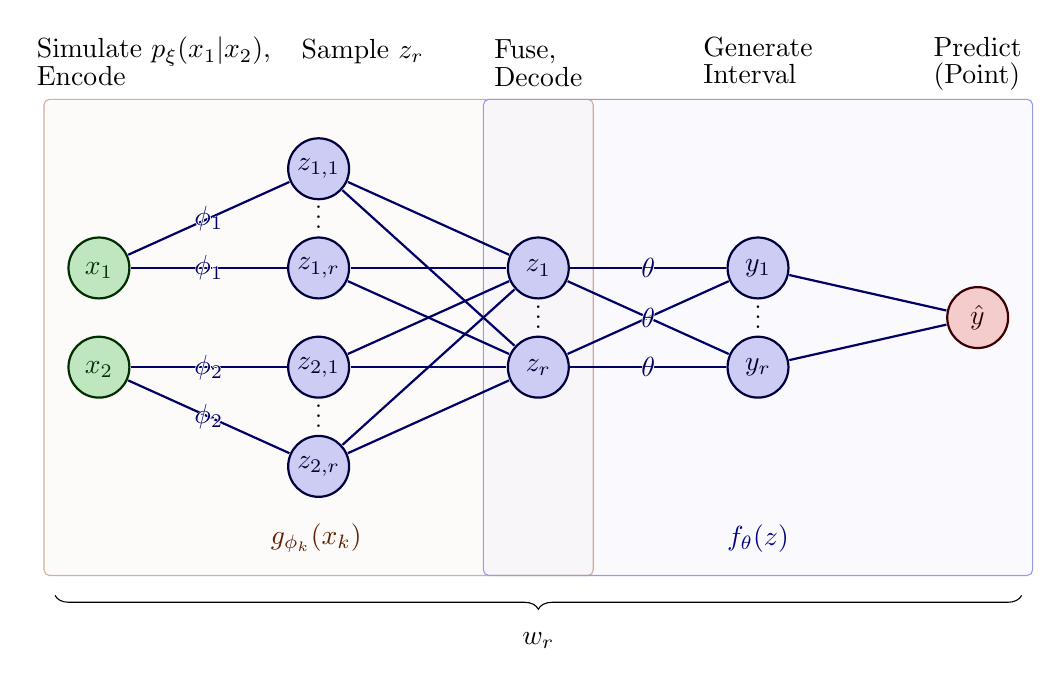
\begin{tikzpicture}[x=3.1cm,y=1.4cm, scale = 0.9]
    \draw[myorange!40,fill=myorange,fill opacity=0.02,rounded corners=2]
        (0.75,-2.3) rectangle++ (2.5,4.8); % Y-coordinates moved up
    \draw[myblue!40,fill=myblue,fill opacity=0.02,rounded corners=2]
        (2.75,-2.3) rectangle++ (2.5,4.8); % Y-coordinates moved up

    \node[right=19,above=3,align=center,myorange!60!black] at (1.75,-2.25) {$g_{\phi_k}(x_k)$};
    \node[above=3,align=center,myblue!60!black] at (4,-2.25) {$f_{\theta}(z)$};
    
  \readlist\Nnod{2,4,2,2,1} % array of number of nodes per layer
  \readlist\Cstr{\strut x,z, z,y,\hat{y}} % array of coefficient symbol per layer
  \readlist\Nstr{2,{,},r,r,} % array of string number of nodes per layer, with 1,2 for the x nodes
  \readlist\CstrN{\strut x,\phi,,\theta,} % array of coefficient symbol per layer
  % \def\yshift{0} % shift last node for dots

% Define the number of z nodes that each x node should connect to
\newcommand{\numZPerX}{2} % Set this to the number of z nodes for each x node

% Loop over layers
\foreachitem \N \in \Nnod{
    \def\lay{\Ncnt} % Index of current layer
    \pgfmathsetmacro\prev{int(\Ncnt-1)} % Index of previous layer
    
    % Draw nodes with appropriate subscripts
    \foreach \i [evaluate={
                 \c=int(\i==\N);
                 \y=\boxcenter + (\N/2-\i)*1 - \c*\yshift; % Adjust y-coordinates based on the box center
                 \index=(\i<\N?int(\i):"\Nstr[\lay]");
                 \x=\lay; \n=\nstyle;
                }] in {1,...,\N}{

        % Special subscript for the z nodes in the second layer
        \ifnum\lay=2
            % Calculate the x subscript
            \pgfmathtruncatemacro{\xsub}{int((\i+1)/\numZPerX)}
            % Calculate the z subscript
            \pgfmathtruncatemacro{\zsub}{int(mod(\i-1,\numZPerX)+1)}
            % Determine the second subscript
            \ifnum\zsub=1
                \def\zsubscript{1} % First z node gets a subscript of 1
            \else
                \def\zsubscript{r} % Second z node gets a subscript of r
            \fi
            % Use k for the last set of z nodes
            \ifnum\xsub=\Nnod[1]
                \node[node \n] (N\lay-\i) at (\x,\y) {$z_{\xsub,\zsubscript}$};
            \else
                \node[node \n] (N\lay-\i) at (\x,\y) {$z_{\xsub,\zsubscript}$};
            \fi
        \else
            \node[node \n] (N\lay-\i) at (\x,\y) {$\Cstr[\lay]_{\index}$};
        \fi

    % Insert the vertical dots for the second layer between first two nodes
    \ifnum\lay=2
        \ifnum\i=1 % After the first node, but before the second
            % Draw the vertical dots
            \path (N\lay-\i) --++ (0,-0.5) node[midway,scale=0.9] {$\vdots$};
        \fi
    \fi
    
    % Add this line just before drawing the last node in each layer
    % Check if it's not the first two layers, nor the last layer
    \ifnum\lay>1
      \ifnum\lay<\Nnodlen
        \ifnum\i=\N
          \path (N\lay-\N) --++ (0,0.835) node[midway,scale=0.9] {$\vdots$};
        \fi
      \fi
    \fi
    }

    % Draw connections
    \ifnum\lay>1
        \foreach \j in {1,...,\Nnod[\prev]}{
            \ifnum\lay=2
                % Draw connections from x to z nodes with phi labels
              \foreach \i in {1,...,\numZPerX}{
                  \pgfmathtruncatemacro{\targetindex}{(\j - 1) * \numZPerX + \i}
                  % Check if we are at the last x node to assign phi_k
                  \ifnum\j=\Nnod[1]
                      \draw[connect] (N1-\j) -- (N2-\targetindex)
                          node[pos=0.50]{\contour{white}{$\phi_2$}}; % Use phi_k for the last x node
                  \else
                      \draw[connect] (N1-\j) -- (N2-\targetindex)
                          node[pos=0.50]{\contour{white}{$\phi_{\j}$}}; % phi with subscript
                  \fi
              }
            \else
                \ifnum\lay=4
                    % Draw connections from z to y nodes with theta labels
                    \foreach \i in {1,...,\N}{
                        \draw[connect] (N\prev-\j) -- (N\lay-\i)
                            node[midway, pos=0.50] {\contour{white}{$\theta$}}; % theta label on the line
                    }
                \else
                    % Draw connections from y to y_hat nodes without labels
                    \foreach \i in {1,...,\N}{
                        \draw[connect] (N\prev-\j) -- (N\lay-\i);
                    }
                \fi
            \fi
        }
    \fi
}

      % % Add the box labels
      % \node[above=10,align=center,black] at (1.5,2.2) {Encoding}; % Between layers 1 and 2
      % \node[above=10,align=center,black] at (3.0,2.25) {Fusion}; % At layer 3
      % \node[above=10,align=center,black] at (4.5,2.2) {Decoding}; % Between layers 4 and 52

      % Add the operation labels
      % \node[above=10,align=left,black] at (1.2,2.26) {Simulate $_{\xi}(\cdot | x_{2})$,\\[-0.2em]Encode}; % Above layer 1
      \node[above=10,align=left,black] at (1.25,2.26) {Simulate $p_{\xi}(x_1 | x_{2})$,\\[-0.2em]Encode}; % Above layer 1
      % \node[above=10,align=left,black] at (2.0,2.2) {Sample $p_{\phi_k}(\cdot | x_{k,r})$,\\[-0.2em] If $x_1$ missing $\sim p_{\xi}(\cdot | x_{k})$}; % Above layer 2
      % \node[above=10,align=left,black] at (2.2,2.2) {Sample $z_{r}$\\[-0.2em]${\cal N}(g_{\phi_k}(x), \sigma_{k}^2)$};
      \node[above=10,align=left,black] at (2.2,2.2) {Sample $z_{r}$\\};
      \node[above=10,align=left,black] at (3.0,2.25) {Fuse,\\[-0.2em]
      Decode}; % Above layer 3
      \node[above=10,align=left,black] at (4.0,2.0) {Generate\\[-0.2em]Interval\\[-0.2em]}; % Above layer 5
      \node[above=10,align=left,black] at (5.0,2.0) {Predict\\[-0.2em](Point)\\[-0.2em]}; % Above layer 5
      
    \draw [decorate,decoration={brace,amplitude=5pt,mirror}] (0.8,-2.5) -- (5.2,-2.5) node [midway,below=10pt] {$w_{r}$}; % Y-coordinate moved up
    
\end{tikzpicture}
\end{minipage}
\end{center} % Add this line to end the center environment

\end{document}